\documentclass[11pt,aspectratio=169]{beamer}

\usetheme{Madrid}
\usecolortheme{seahorse}

\usepackage[utf8]{inputenc}
\usepackage{amsmath,amssymb}
\usepackage{xcolor}
\usepackage{booktabs}
\usepackage{tikz}
\usetikzlibrary{arrows.meta}

\setbeamertemplate{navigation symbols}{}
\setbeamertemplate{footline}[frame number]

\title{Beyond the Syllabus}
\subtitle{Complexity Classes and Three 2024--2025 Breakthroughs in Algorithms\\
\small Week 2 Supplement -- TOAE209/TOAH209: Design and Analysis of Algorithms}
\author{Foreign Trade University}
\date{}

\begin{document}

% ---------------------------------------------------------------
\begin{frame}
  \titlepage
\end{frame}
% ---------------------------------------------------------------

\begin{frame}{Outline}
  \tableofcontents
\end{frame}

% =================================================================
\section{Motivation}
% =================================================================

\begin{frame}{Why look beyond the syllabus?}
  \begin{itemize}
    \item This course teaches you \textbf{tools}: asymptotic analysis, greedy algorithms,
    divide and conquer, dynamic programming, network flow, NP-completeness.
    \item These tools are not museum pieces. Researchers are actively using them
    \textbf{right now} to settle questions that were open for 40--60 years.
    \item Today's supplement has two parts:
    \begin{enumerate}
      \item A map of the \textbf{complexity classes} that organize ``how hard is this
      problem, really?'' -- the language you need to read any theory paper.
      \item Three \textbf{2024--2025 breakthroughs} that each broke a decades-old
      speed barrier, using exactly the kind of reasoning ($T(n) = \ldots$, recurrences,
      worst-case analysis) you are learning this semester.
    \end{enumerate}
  \end{itemize}
  \begin{alertblock}{The message}
    ``Textbook algorithm'' does not mean ``final answer.'' Dijkstra's algorithm is 70 years
    old and still generating Symposium-on-Foundations-of-Computer-Science best-paper awards.
  \end{alertblock}
\end{frame}

% =================================================================
\section{The Landscape of Complexity Classes}
% =================================================================

\begin{frame}{What is a complexity class?}
  \begin{block}{Definition (informal)}
    A \textbf{complexity class} is a set of computational problems that can be solved
    using a certain amount of a resource -- usually \textbf{time} or \textbf{space} --
    as a function of input size $n$.
  \end{block}
  \vspace{0.5em}
  \begin{itemize}
    \item You already know one: this whole course is implicitly about the class of
    problems solvable in \textbf{polynomial time}.
    \item Complexity theory asks a sharper question: \emph{for a given problem, is
    polynomial time enough -- and if we don't know, what can we prove about it anyway?}
    \item This matters practically: if a problem is provably ``hard,'' you stop searching
    for a fast exact algorithm and instead look for approximations, heuristics, or
    special-case structure (topics in Weeks 12--15).
  \end{itemize}
\end{frame}

\begin{frame}{P: efficiently solvable problems}
  \begin{block}{P (Polynomial time)}
    The class of decision problems solvable by an algorithm running in $O(n^k)$ time for
    some constant $k$, on a standard (deterministic) computer.
  \end{block}
  \begin{itemize}
    \item Shortest paths, minimum spanning tree, sorting, matching, network flow -- almost
    everything in Weeks 3--11 of this course lives in P.
    \item ``Polynomial'' is the standard mathematical stand-in for \textbf{``efficient.''}
    $O(n^3)$ can be slow in practice, and $O(1.01^n)$ is technically not polynomial -- but
    the P/not-P line is the most useful coarse-grained boundary theorists have found.
  \end{itemize}
\end{frame}

\begin{frame}{NP: efficiently \emph{verifiable} problems}
  \begin{block}{NP (Nondeterministic Polynomial time)}
    The class of decision problems where, \emph{if the answer is ``yes,''} there exists a
    proof (a \textbf{certificate}) that can be \textbf{checked} in polynomial time.
  \end{block}
  \begin{itemize}
    \item Example: ``Does this graph have a Hamiltonian cycle?'' Nobody knows how to
    \emph{find} one quickly, but if someone hands you a candidate cycle, you can
    \emph{verify} it visits every vertex exactly once in $O(n)$ time.
    \item Every problem in P is also in NP (if you can solve it fast, you can certainly
    verify a solution fast): $\mathbf{P \subseteq NP}$.
    \item The single biggest open question in computer science: \textbf{is $P = NP$?}
    Can everything that's easy to \emph{check} also be made easy to \emph{solve}?
  \end{itemize}
\end{frame}

\begin{frame}{NP-complete and NP-hard}
  \begin{itemize}
    \item A problem is \textbf{NP-hard} if every problem in NP can be reduced to it in
    polynomial time -- informally, it is ``at least as hard as anything in NP.''
    \item A problem is \textbf{NP-complete} if it is NP-hard \emph{and} itself in NP.
    NP-complete problems are the ``hardest problems inside NP.''
    \item Cook and Levin (1971) showed \textsc{SAT} (Boolean satisfiability) is
    NP-complete. Thousands of problems are now known to be NP-complete, including
    the \textbf{Traveling Salesman Problem} (decision version), \textsc{3-Coloring}, and
    \textsc{Vertex Cover} -- you will meet several of these formally in Week 12.
  \end{itemize}
  \begin{exampleblock}{Why this matters in practice}
    If you can reduce a known NP-complete problem to \emph{your} problem, you have strong
    evidence your problem has \textbf{no} polynomial-time exact algorithm (unless $P=NP$).
    That is your cue to switch strategies: approximation (Week 14), randomization
    (Week 15), or exponential-but-practical search.
  \end{exampleblock}
\end{frame}

\begin{frame}{The big picture}
  \begin{center}
  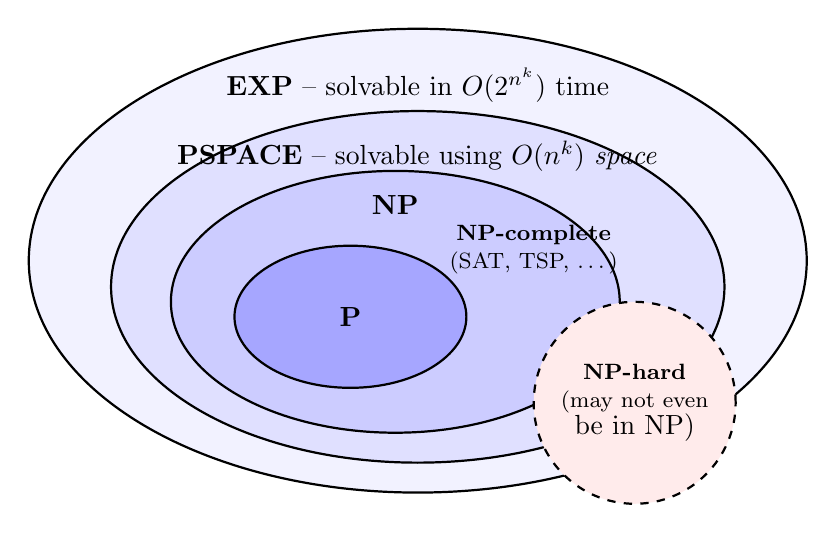
\begin{tikzpicture}[scale=0.95]
    \draw[thick, fill=blue!5] (0,0) ellipse (5.2 and 3.1);
    \node at (0,2.35) {\textbf{EXP} -- solvable in $O(2^{n^k})$ time};

    \draw[thick, fill=blue!12] (0,-0.35) ellipse (4.1 and 2.35);
    \node at (0,1.4) {\textbf{PSPACE} -- solvable using $O(n^k)$ \emph{space}};

    \draw[thick, fill=blue!20] (-0.3,-0.55) ellipse (3.0 and 1.75);
    \node at (-0.3,0.75) {\textbf{NP}};

    \draw[thick, fill=blue!35] (-0.9,-0.75) ellipse (1.55 and 0.95);
    \node at (-0.9,-0.75) {\textbf{P}};

    \node[align=center] at (1.55,0.15) {\footnotesize \textbf{NP-complete}\\[-2pt]
      \footnotesize (SAT, TSP, \ldots)};

    \draw[thick, dashed, fill=red!8] (2.9,-1.9) circle (1.35);
    \node[align=center] at (2.9,-1.9) {\footnotesize \textbf{NP-hard}\\[-2pt]
      \footnotesize (may not even\\[-2pt] be in NP)};
  \end{tikzpicture}
  \end{center}
  \begin{itemize}
    \item Known for sure: $\mathbf{P \subseteq NP \subseteq PSPACE \subseteq EXP}$.
    \item \textbf{Not} known: whether any of these inclusions is \emph{strict}. (One is:
    $P \ne EXP$, by a classical diagonalization argument -- but where the gap actually
    lives is wide open.)
  \end{itemize}
\end{frame}

\begin{frame}{P vs.\ NP: the \$1{,}000{,}000 question}
  \begin{itemize}
    \item $P$ vs.\ $NP$ is one of the seven \textbf{Clay Millennium Prize Problems}
    (\$1{,}000{,}000 for a correct proof either way). Only one Millennium Problem has
    been solved so far (the Poincar\'e conjecture, by Grigori Perelman, 2003).
    \item Almost every theorist believes $P \ne NP$ -- but belief is not proof, and the
    problem has resisted every attack for over 50 years.
    \item \textbf{Why you should care as a 2nd-year student:} every time you face a new
    problem in industry or research, ``is this secretly NP-hard?'' is one of the first
    questions worth asking, \emph{before} you spend a week trying to write a fast
    exact algorithm.
  \end{itemize}
  \begin{alertblock}{Looking ahead}
    Week 12 makes all of this precise: formal reductions, Cook--Levin, and a toolkit for
    proving your own problems NP-hard.
  \end{alertblock}
\end{frame}

% =================================================================
\section{Recent Advances I: Matrix Multiplication After Strassen}
% =================================================================

\begin{frame}{Recap: Strassen's trick (1969)}
  \begin{itemize}
    \item You saw last week that Karatsuba traded one multiplication for extra additions
    to beat the $\Theta(n^2)$ grade-school bound.
    \item Volker Strassen applied the \emph{same philosophy} to \textbf{matrix
    multiplication}: multiplying two $2\times 2$ block matrices needs only \textbf{7}
    multiplications (of the blocks), not the obvious \textbf{8}.
    \item Recursively applied to $n\times n$ matrices:
    \[
      T(n) = 7\,T(n/2) + O(n^2) \;\Longrightarrow\; T(n) = \Theta(n^{\log_2 7}) \approx
      \Theta(n^{2.807}),
    \]
    beating the schoolbook $\Theta(n^3)$ -- the first improvement in recorded history.
  \end{itemize}
\end{frame}

\begin{frame}{The exponent $\omega$: a 50-year race}
  Define $\omega$ as the smallest exponent such that $n\times n$ matrices can be
  multiplied in $O(n^{\omega+\varepsilon})$ time for every $\varepsilon > 0$.
  \begin{center}
  \begin{tabular}{@{}lll@{}}
    \toprule
    Year & Result & Bound on $\omega$ \\
    \midrule
    1969 & Strassen & $2.807\ldots$ \\
    1990 & Coppersmith--Winograd & $2.376$ \\
    2014 & Le Gall & $2.3728639$ \\
    2020--21 & Alman--Williams & $2.3728596$ \\
    2022 & Duan--Wu--Zhou & $2.3719$ \\
    2024 & Williams--Xu--Xu--Zhou & $2.371339$ \\
    \bottomrule
  \end{tabular}
  \end{center}
  \begin{itemize}
    \item Nobody knows the true value of $\omega$; many suspect $\omega = 2$ is
    achievable, but every attempt to prove it has stalled.
    \item These are all \textbf{asymptotic} (large-$n$) results with enormous constants --
    not (yet) practical for the matrix sizes you'd use in a homework assignment.
  \end{itemize}
\end{frame}

\begin{frame}{A different question: the small-case puzzle}
  \begin{itemize}
    \item Separately from the asymptotic race, there is a very concrete combinatorial
    question: \textbf{exactly how many scalar multiplications are needed to multiply
    two $4\times 4$ matrices?}
    \item Applying Strassen recursively to a $4\times 4$ matrix (as two levels of
    $2\times 2$ blocks) uses $7\times 7 = \mathbf{49}$ multiplications.
    \item For over 50 years, \textbf{49} was the best known scheme for $4\times 4$
    matrices -- until 2022.
  \end{itemize}
  \begin{block}{Why anyone cares about ``49 vs.\ 47''}
    Small building blocks get used \emph{recursively}. Shaving multiplications off the
    base case improves the constant in the asymptotic bound every level of recursion --
    exactly like the jump from 4 to 3 recursive calls did for Karatsuba.
  \end{block}
\end{frame}

\begin{frame}{AI-assisted discovery joins the search}
  \begin{center}
  \begin{tabular}{@{}lll@{}}
    \toprule
    Year & Who / what & Result for $4\times 4$ \\
    \midrule
    1969--2021 & Strassen (recursive) & 49 multiplications \\
    2022 & DeepMind's \textbf{AlphaTensor} & 47 multiplications (mod-2 arithmetic) \\
    2024 & Kauers \& Moosbauer (JKU Linz) & 48 multiplications (standard arithmetic) \\
    2025 & DeepMind's \textbf{AlphaEvolve} & 48 multiplications (complex-valued) \\
    \bottomrule
  \end{tabular}
  \end{center}
  \vspace{0.5em}
  \begin{itemize}
    \item AlphaTensor (Nature, 2022) reframed matrix multiplication as a single-player
    game and used reinforcement learning to search for low-multiplication schemes --
    the first improvement on Strassen's 4x4 case in 55 years.
    \item AlphaEvolve (2025) is a large-language-model-driven \emph{evolutionary code
    search}: it proposes, tests, and refines algorithm implementations directly.
  \end{itemize}
  \begin{alertblock}{The lesson}
    A problem being ``settled since 1969'' didn't mean it was actually settled --
    it meant nobody had looked hard enough, with the right tools.
  \end{alertblock}
\end{frame}

% =================================================================
\section{Recent Advances II: Shortest Paths Beyond Dijkstra}
% =================================================================

\begin{frame}{Dijkstra's algorithm (1956) and the sorting barrier}
  \begin{itemize}
    \item \textbf{Single-source shortest paths:} given a graph with $n$ vertices, $m$
    edges, and a source $s$, find the shortest distance from $s$ to every other vertex.
    \item Dijkstra's algorithm: repeatedly pick the \emph{closest unvisited} vertex,
    ``finalize'' its distance, and relax its outgoing edges.
    \item In 1984, Fredman and Tarjan's \textbf{Fibonacci heap} made this run in
    $O(m + n\log n)$ time -- matching a fundamental lower bound: any algorithm that
    finalizes vertices \emph{in sorted order of distance} cannot beat the time it takes
    to \textbf{sort} $n$ numbers.
  \end{itemize}
  \begin{exampleblock}{The ``sorting barrier''}
    For 40 years, this looked like the end of the road for general (real-weighted)
    graphs -- \emph{unless} you find a way to avoid sorting altogether.
  \end{exampleblock}
\end{frame}

\begin{frame}{2024: Dijkstra is ``universally optimal''}
  \begin{itemize}
    \item Haeupler, Rozho\v{n}, T\v{e}tek, Hladík, and Tarjan (\textsc{FOCS} 2024 best
    paper) asked a different question: not ``what is the worst case over \emph{all}
    graphs,'' but \textbf{``is there one algorithm that is the best possible on
    \emph{every individual} graph structure?''}
    \item They designed a new heap data structure and proved: a variant of Dijkstra's
    algorithm is \textbf{universally optimal} -- for every fixed graph \emph{shape},
    no algorithm can beat it (for worst-case edge weights on that shape).
    \item A beautiful, 70-years-later vindication of Dijkstra's original 20-minute,
    pencil-free design.
  \end{itemize}
\end{frame}

\begin{frame}{2025: breaking the sorting barrier}
  \begin{itemize}
    \item Just one year later, Duan, Mao, and collaborators (\textsc{STOC} 2025 best
    paper) proved the opposite-sounding result: an algorithm that
    \textbf{beats} Dijkstra's $O(m + n\log n)$ \emph{worst-case} bound, on general
    directed, real-weighted graphs.
    \item Key idea: don't finalize vertices strictly by increasing distance.
    \begin{itemize}
      \item Group nearby frontier vertices into \textbf{clusters}; explore one
      representative per cluster instead of scanning the whole frontier.
      \item Use short, bounded bursts of the (usually slow) \textbf{Bellman--Ford}
      algorithm to find ``influential'' hub vertices worth exploring next.
    \end{itemize}
    \item Because vertices are no longer finalized in sorted order, the sorting lower
    bound simply \textbf{does not apply} to this algorithm.
  \end{itemize}
\end{frame}

\begin{frame}{Reconciling the two results}
  \begin{center}
  \begin{tabular}{@{}p{4.6cm}p{4.6cm}@{}}
    \toprule
    \textbf{2024 (Haeupler et al.)} & \textbf{2025 (Duan, Mao et al.)} \\
    \midrule
    ``Best possible \emph{per graph shape},'' among algorithms that finalize vertices
    by increasing distance & ``Faster \emph{in the worst case over all graphs},''
    by abandoning distance-order finalization entirely \\
    \bottomrule
  \end{tabular}
  \end{center}
  \vspace{0.5em}
  \begin{alertblock}{The teaching moment}
    Both statements are true. ``Optimal'' always means \emph{optimal with respect to a
    model and a metric}. Changing the model (what the algorithm is allowed to do) or the
    metric (worst-case-over-graphs vs.\ per-graph-shape) can change the answer --
    a theme you will see again with approximation ratios in Week 14.
  \end{alertblock}
\end{frame}

% =================================================================
\section{Recent Advances III: Coloring Graphs Near-Optimally}
% =================================================================

\begin{frame}{The problem: edge coloring}
  \begin{itemize}
    \item \textbf{Motivating story:} at an airport, model runways/taxiways/gates as
    vertices and each aircraft's planned route as a path connecting them. Color each
    edge (route segment) so that no two edges sharing a vertex share a color -- colors
    represent non-conflicting time slots.
    \item \textbf{Vizing's theorem} (1964): every graph can be edge-colored with at most
    $\Delta + 1$ colors, where $\Delta$ is the maximum vertex degree. Knowing \emph{how
    many} colors suffice is easy.
    \item \textbf{Actually finding} such a coloring quickly is a different, much harder
    story.
  \end{itemize}
\end{frame}

\begin{frame}{A 40-year plateau}
  \begin{itemize}
    \item Vizing's own algorithm runs in $O(mn)$ time (recoloring a chain of edges can
    cascade across the whole graph).
    \item 1980s improvements brought this down to $O(m\sqrt n)$ -- and then progress
    \textbf{stalled for roughly 40 years}.
    \item ``The research stopped for a very long time \ldots\ many people believed that
    there's no better way,'' as one researcher put it.
  \end{itemize}
\end{frame}

\begin{frame}{2024--2025: near-linear time, finally}
  \begin{itemize}
    \item 2024: two independent groups broke the 40-year plateau within days of each
    other: Assadi's $O(n^2)$-time algorithm, and a separate $O(m\sqrt[3]{n})$-time
    algorithm, later refined to $O(m\sqrt[4]{n})$.
    \item 2025: Assadi, Behnezhad, Costa, and collaborators combined forces and went
    much further -- a \textbf{near-linear} $O(m\log m)$-time algorithm, presented at
    \textsc{STOC} 2025.
    \item Since simply \emph{reading} the graph takes $\Omega(m)$ time, $O(m\log m)$ is
    within a single logarithmic factor of the \textbf{theoretical minimum possible}.
  \end{itemize}
  \begin{block}{The key new idea: ``priming''}
    Rather than trying to color the \emph{last, hardest} edge faster (the old approach),
    use randomization to color \emph{almost all} edges at once, leaving only a small,
    structured set of edges -- which can then be colored quickly and nearly
    simultaneously.
  \end{block}
\end{frame}

\begin{frame}{Why these three stories matter}
  \begin{itemize}
    \item Every one of these breakthroughs attacks a \textbf{classical, textbook}
    problem: matrix multiplication, shortest paths, edge coloring.
    \item Every one of these barriers stood for \textbf{decades} (40--55 years) and was
    widely believed to be permanent.
    \item Every one of these breakthroughs came from a genuinely \textbf{new idea} about
    combining old techniques (clustering, bounded Bellman--Ford bursts, randomized
    ``priming''), not from more computing power alone -- though AI-assisted search
    (AlphaTensor, AlphaEvolve) is now a serious new tool in the theorist's toolbox.
  \end{itemize}
\end{frame}

% =================================================================
\section{Summary}
% =================================================================

\begin{frame}{Summary}
  \begin{enumerate}
    \item \textbf{Complexity classes} (P, NP, NP-complete, NP-hard, PSPACE, EXP) give you
    a vocabulary for asking ``how hard, provably, is this problem?'' -- $P$ vs.\ $NP$
    remains the field's central open question.
    \item \textbf{Matrix multiplication:} the asymptotic exponent $\omega$ keeps
    inching down (2.807 $\to$ 2.371), and AI-assisted search (AlphaTensor,
    AlphaEvolve) has now improved even the small, 55-year-old $4\times 4$ case.
    \item \textbf{Shortest paths:} Dijkstra's algorithm was proved \emph{universally
    optimal} in 2024 -- and its worst-case bound was still \emph{beaten} in 2025, by
    an algorithm that refuses to sort. Both are correct; they optimize different things.
    \item \textbf{Edge coloring:} a 40-year-stalled problem fell to near-linear time in
    2024--2025 via a new ``priming'' idea.
  \end{enumerate}
  \begin{alertblock}{Looking ahead}
    The tools behind every one of these results -- recurrences, worst-case analysis,
    reductions, randomization -- are exactly what the rest of this course builds up,
    week by week.
  \end{alertblock}
\end{frame}

\end{document}
